\chapter{beatific bursts} 
\label{sec:bursts}
\rhead[]{\leftmark}
\lstset{style=6502Style}
Bursts are short pre-programmed sequences of patterns that can be invoked using the Function keys.
This allows the player to define up to four different burst sequences, one per function key. A burst
can consist of up to 16 different patterns displayed in 16 different positions on the screen. Each burst
has a defined symmetry and smoothing delay. The greater the smoothing delay, the longer the pattern
will stay on screen.

The bursts are programmable, the player can define new ones through the slightly finicky process of pressing
Shift and the corresponding Function key, then selecting the different points on the screen for each of up
to 16 patterns to appear. You can see the data structure that supports this on the following page. Note
that the symmetry and smoothing delay are set for the burst sequence as a whole, but each element of the
burst sequence has its own pattern and position co-ordinates.

\clearpage
\begin{figure}[H]
    \centering
    \begin{adjustbox}{width=12cm,center}
      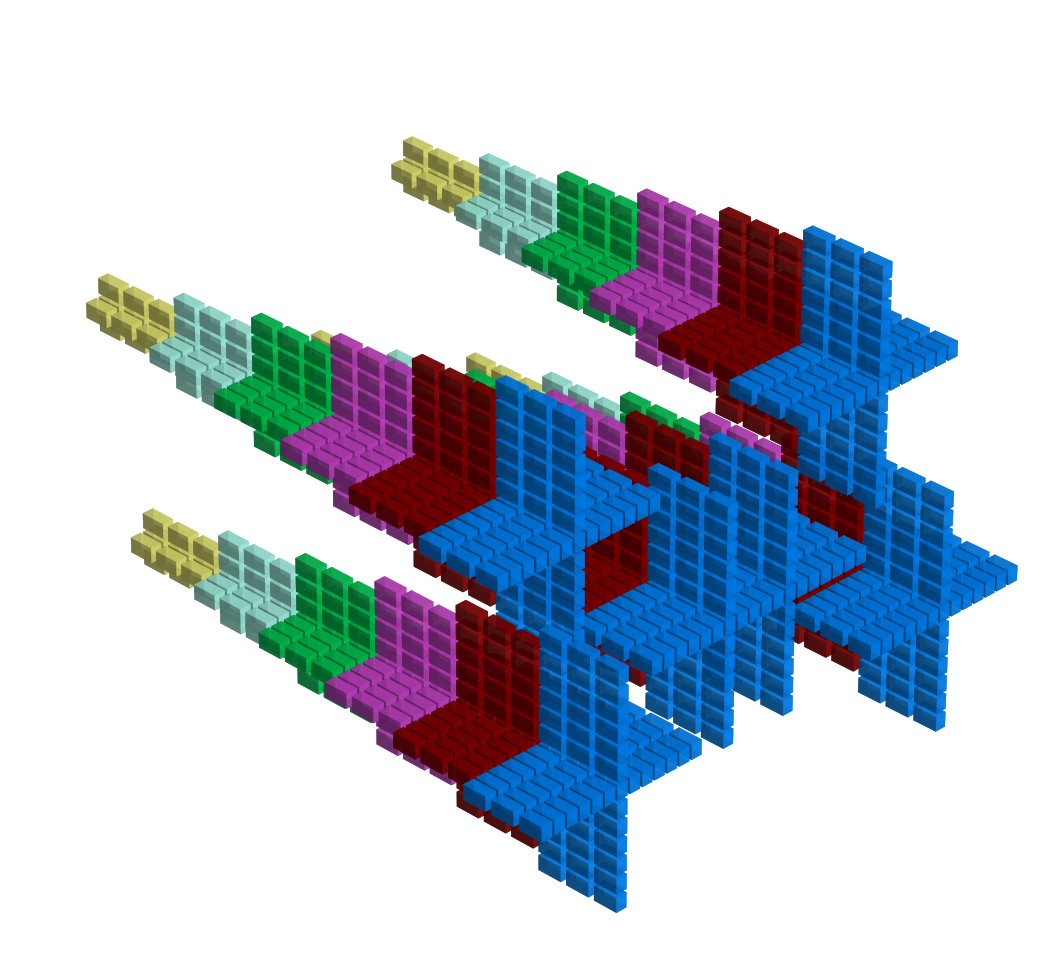
\includegraphics[width=12cm]{src/patterns/bursts/pattern0-45.png}%
    \end{adjustbox}
\caption{Evolution of the default burst at F1.}
\end{figure}
\clearpage

\rhead[]{F1 Burst}
\begin{lstlisting}[caption=Source code for the F1 Burst.]
burstGeneratorF1 = $C200
  ; currentSymmetrySetting: 'Current symmetry setting.'
  ; Possible values are 0 - 4:
  ; 'NO SYMMETRY     '
  ; 'Y-AXIS SYMMETRY '
  ; 'X-Y SYMMETRY    '
  ; 'X-AXIS SYMMETRY '
  ; 'QUAD SYMMETRY   '
  .BYTE $01
  ; smoothingDelay: 'Because of the time taken to draw larger patterns
  ; speed increase-decrease is not linear. You can adjust the 
  ; compensating delay which often smooths out jerky patterns. 
  ; Can be used just for special FX) though. Suck it and see.'
  .BYTE $0C

  ; Burst Position 1
  ; X/Y Co-ordinates: X/Y Position relative to cursor to place the
  ; burst.
  .BYTE $07,$06
  ; Index to pattern in patternIndexArray
  .BYTE PULSAR

  ; Burst Position 2
  ; X/Y Co-ordinates: X/Y Position relative to cursor to place the
  ; burst.
  .BYTE $11,$0D
  ; Index to pattern in patternIndexArray
  .BYTE PULSAR

  ; Burst Position 3
  ; X/Y Co-ordinates: X/Y Position relative to cursor to place the 
  ; burst.
  .BYTE $06,$11
  ; Index to pattern in patternIndexArray
  .BYTE PULSAR

  ; - An $FF in the first byte of 'X/y Co-ordinates' indicates the
  ; end of the data, e.g. in 'Burst Position 4' below.
  ; Burst Position 4
  ; X/Y Co-ordinates: X/Y Position relative to cursor to place the 
  ; burst.
  .BYTE $FF,$0B
  ; Index to pattern in patternIndexArray
  .BYTE PULSAR

\end{lstlisting}

\clearpage
\begin{lstlisting}
functionKeys .BYTE $04,$05,$06,$03
;-------------------------------------------------------
; CheckKeyboardInput
;-------------------------------------------------------
CheckKeyboardInput   
        ...

        ; Was one of the function keys pressed?
MaybeFunctionKeysPressed   
        LDX #$00
FnKeyLoop   
        CMP functionKeys,X
        BEQ FunctionKeyWasPressed ; One of them was pressed!
        INX 
        CPX #$04
        BNE FnKeyLoop
        ; Continue checking
        JMP MaybeQPressed

        ; A Function key was pressed, ignore if the sequencer is active.
FunctionKeyWasPressed   
        STX functionKeyIndex
        LDA sequencerActive
        BNE MaybeQPressed
        LDA #SEQUENCER_ACTIVE
        STA currentVariableMode
        JSR LoadOrProgramBurstGenerator
        RTS 
\end{lstlisting}
\clearpage

\rhead[]{\icode{CheckKeyboardInput}}
\begin{wrapfigure}{r}{0.15\textwidth}
\frame{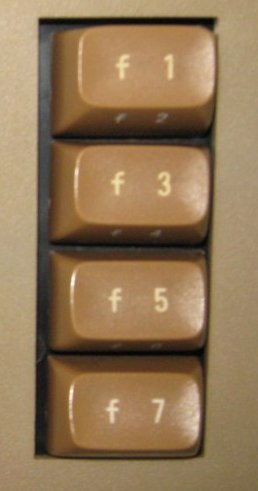
\includegraphics[width=2cm]{src/bursts/fn_keys_only.jpg}}%
\end{wrapfigure}
\textbf{Lines 1189-1231. \icode{\textbf{CheckKeyboardInput}}:} This is the routine that detects when the player has selected a new
Burst by pressing one of the four 'Function' keys. It is part of the much larger routine \icode{CheckKeyboardInput} which periodically checks
for keyboard input by polling the byte at address \icode{\$00C5} (which we label \icode{lastKeyPressed}). This address always
contains the value of the most recently pressed key on the keyboard.

If a valid 'Function' key was pressed the routine calls \icode{LoadOr\-ProgramBurstGenerator}. This routine
will check whether 'Shift' was also pressed. If so, it it will enable the user to program a new
Burst sequence, otherwise it will load the preprogrammed burst sequence associated with the function key.
If a valid 'Function' key was pressed the routine calls \icode{LoadOr\-ProgramBurstGenerator}. This routine
will check whether 'Shift' was also pressed. If so, it it will enable the user to program a new
Burst sequence, otherwise it will load the preprogrammed burst sequence associated with the function key.

\clearpage
\begin{figure}[H]
    \centering
    \begin{adjustbox}{width=12cm,center}
      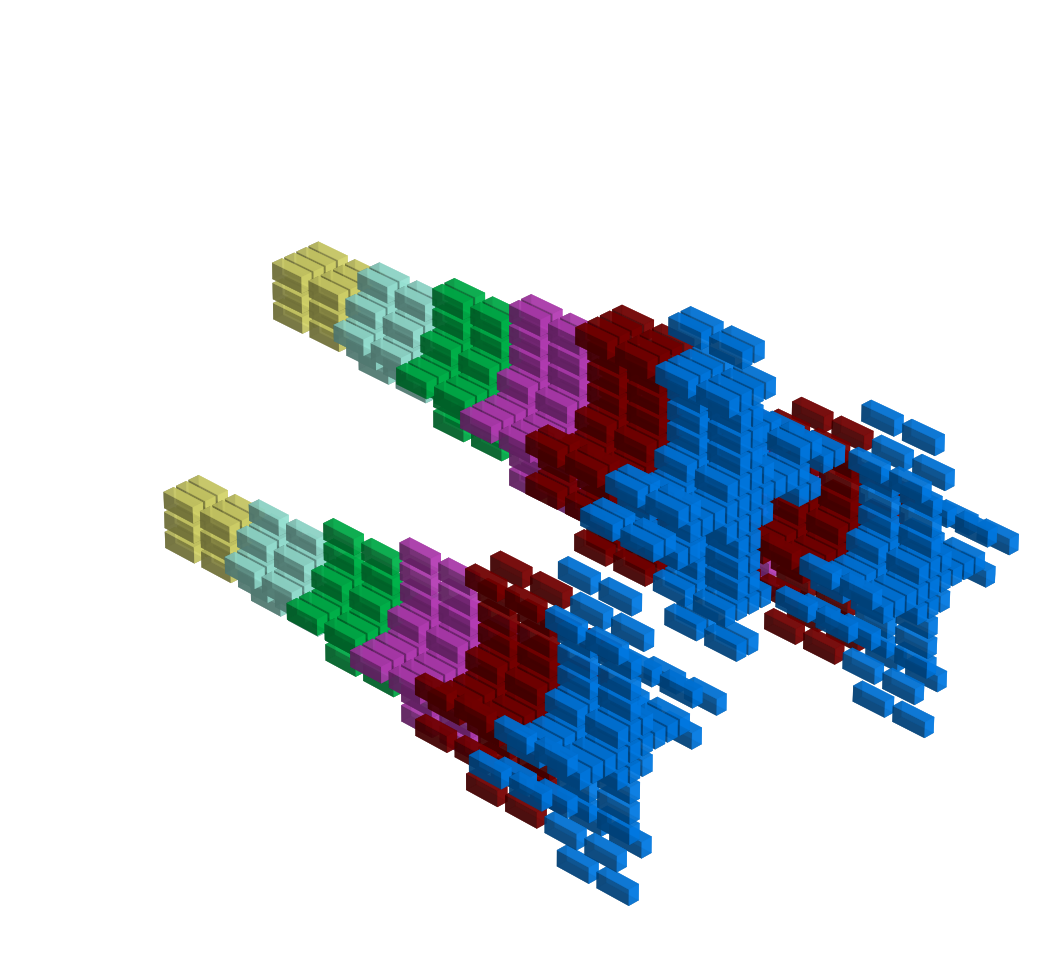
\includegraphics[width=12cm]{src/patterns/bursts/pattern1-45.png}%
    \end{adjustbox}
\caption{Evolution of the default burst at F3.}
\end{figure}
\clearpage

\rhead[]{F3 Burst}
\begin{lstlisting}[caption=Source code for the F3 Burst.]
burstGeneratorF3 = $C220
  ; currentSymmetrySetting: 'Current symmetry setting.'
  ; Possible values are 0 - 4:
  ; 'NO SYMMETRY     '
  ; 'Y-AXIS SYMMETRY '
  ; 'X-Y SYMMETRY    '
  ; 'X-AXIS SYMMETRY '
  ; 'QUAD SYMMETRY   '
  .BYTE Y_AXIS_SYMMETRY

  ; smoothingDelay: 'Because of the time taken to draw larger patterns
  ; speed increase/decrease is not linear. You can adjust the 
  ; compensating delay which often smooths out jerky patterns.
  ; Can be used just for special FX) though. Suck it and see.'
  .BYTE $0C

  ; Burst Position 1
  ; X/Y Co-ordinates: X/Y Position relative to cursor to place burst.
  .BYTE $13,$08
  ; Index to pattern in patternIndexArray
  .BYTE STARONE

  ; Burst Position 2
  ; X/Y Co-ordinates: X/Y Position relative to cursor to place burst.
  .BYTE $07,$0F
  ; Index to pattern in patternIndexArray
  .BYTE STARONE

  ; Burst Position 3
  ; X/Y Co-ordinates: X/Y Position relative to cursor to place burst.
  .BYTE $FF,$00
  ; Index to pattern in patternIndexArray
  .BYTE MULTICROSS

\end{lstlisting}

\clearpage
\begin{lstlisting}
functionKeyToSequenceArray
       .BYTE <burstGeneratorF1,<burstGeneratorF3
       .BYTE <burstGeneratorF5,<burstGeneratorF7
;-------------------------------------------------------
; LoadOrProgramBurstGenerator
;-------------------------------------------------------
LoadOrProgramBurstGenerator   
        JSR ClearLastLineOfScreen
        LDA shiftPressed
        AND #$01
        BEQ PointToBurstData

        ; Display data free
        LDX #$00
b1748   LDA txtDataFree,X
        STA lastLineBufferPtr,X
        INX 
        CPX #$10
        BNE b1748
        JSR WriteLastLineBufferToScreen

PointToBurstData   
        LDA #>burstGeneratorF1
        STA currentSequencePtrHi
        LDX functionKeyIndex
        LDA functionKeyToSequenceArray,X
        STA currentSequencePtrLo

        LDA shiftPressed
        AND #$01
        BEQ LoadBurstDataInstead

        ; Set the current data free to 16
        LDA #$10
        STA currentDataFree

        ; Store the current symmetry setting and smoothing delay
        ; in the storage selected by the function key. 
        LDY #$00
        LDA currentSymmetrySetting
        STA (currentSequencePtrLo),Y
        LDA smoothingDelay
        INY 
        STA (currentSequencePtrLo),Y
        RTS 

LoadBurstDataInstead
        LDA #$FF
        STA sequencerActive
        JMP LoadBurstData

\end{lstlisting}
\clearpage

\rhead[]{\icode{LoadOrProgramBurstGenerator}}
\textbf{Lines 1189-1231. \icode{\textbf{LoadOrProgramBurstGenerator}}:} 
\clearpage

\clearpage
\begin{figure}[H]
    \centering
    \begin{adjustbox}{width=12cm,center}
      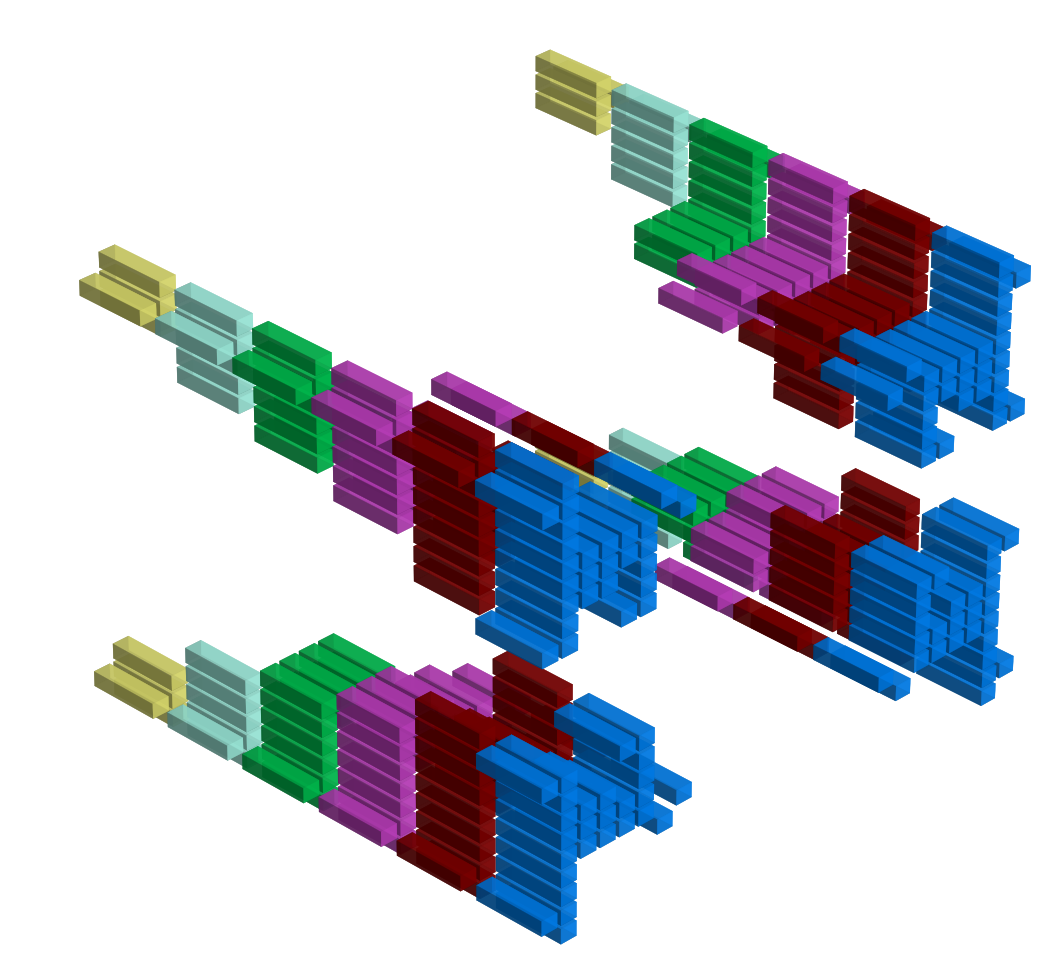
\includegraphics[width=12cm]{src/patterns/bursts/pattern2-45.png}%
    \end{adjustbox}
\caption{Evolution of the default burst at F5.}
\end{figure}
\clearpage

\rhead[]{F5 Burst}
\begin{lstlisting}[caption=Source code for the F5 Burst.]
burstGeneratorF5 = $C240
      ; currentSymmetrySetting: 'Current symmetry setting.'
      ; Possible values are 0 - 4:
      ; 'NO SYMMETRY     '
      ; 'Y-AXIS SYMMETRY '
      ; 'X-Y SYMMETRY    '
      ; 'X-AXIS SYMMETRY '
      ; 'QUAD SYMMETRY   '
      .BYTE QUAD_SYMMETRY
      ; smoothingDelay: 'Because of the time taken to draw larger patterns speed
      ; increase/decrease is not linear. You can adjust the compensating delay
      ; which often smooths out jerky patterns. Can be used just for special FX)
      ; though. Suck it and see.'
      .BYTE $01

      ; Burst Position 1  
      ; X/Y Co-ordinates: X/Y Position relative to cursor to place the burst.
      .BYTE $08,$01
      ; Index to pattern in patternIndexArray
      .BYTE LALLAMITA

      ; Burst Position 2
      ; X/Y Co-ordinates: X/Y Position relative to cursor to place the burst.
      .BYTE $FF,$01
      ; Index to pattern in patternIndexArray
      .BYTE LALLAMITA

\end{lstlisting}

\clearpage
\rhead[]{F7 Burst}
\begin{figure}[H]
    \centering
    \begin{adjustbox}{width=12cm,center}
      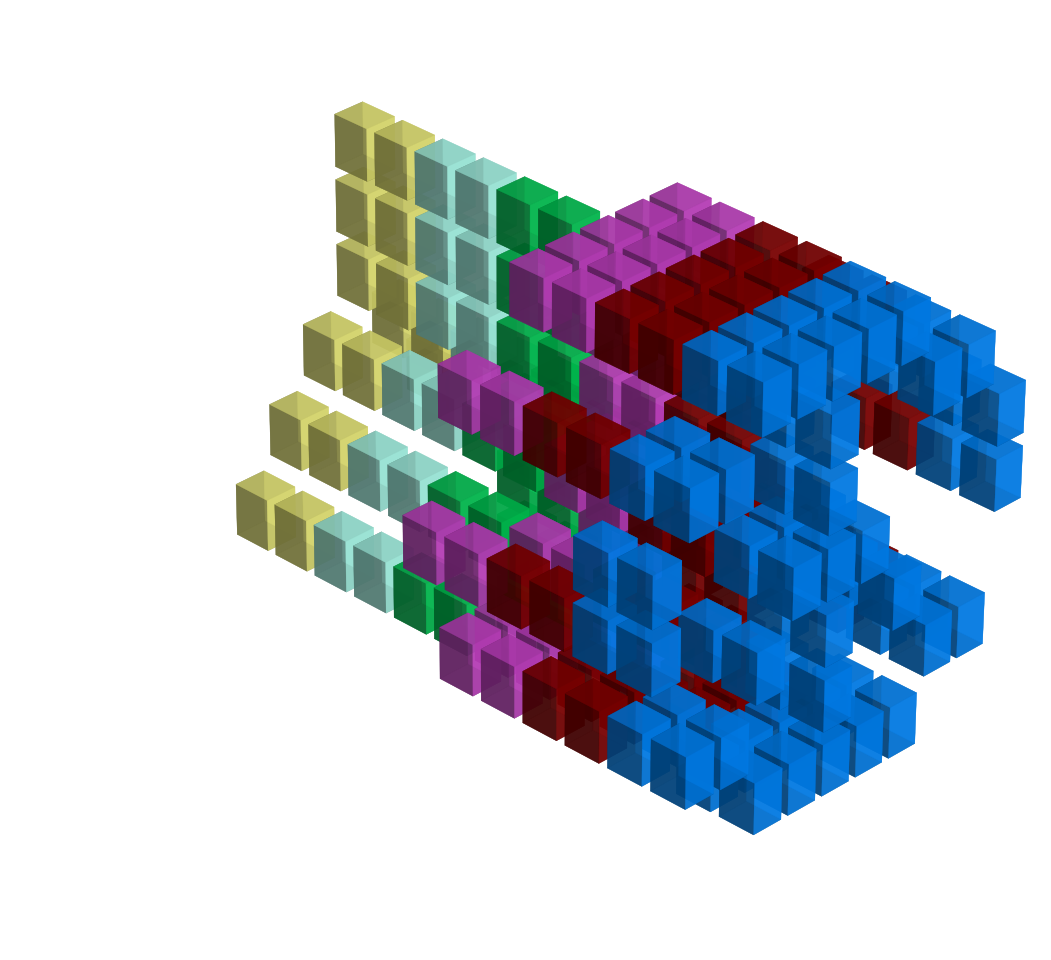
\includegraphics[width=12cm]{src/patterns/bursts/pattern3-45.png}%
    \end{adjustbox}
\caption{Evolution of the default burst at F7.}
\end{figure}
\clearpage

\rhead[]{F7 Burst}
\begin{lstlisting}[caption=Source code for the F7 Burst.]
burstGeneratorF7 = $C260
  ; currentSymmetrySetting: 'Current symmetry setting.'
  ; Possible values are 0 - 4:
  ; 'NO SYMMETRY     '
  ; 'Y-AXIS SYMMETRY '
  ; 'X-Y SYMMETRY    '
  ; 'X-AXIS SYMMETRY '
  ; 'QUAD SYMMETRY   '
  .BYTE NO_SYMMETRY
  ; smoothingDelay: 'Because of the time taken to draw larger patterns
  ; speed increase-decrease is not linear. You can adjust the 
  ; compensating delay which often smooths out jerky patterns. 
  ; Can be used just for special FX) though. Suck it and see.'
  .BYTE $11

  ; Burst Position 1
  ; X/Y Co-ordinates: X/Y Position relative to cursor to place burst.
  .BYTE $12,$09
  ; Index to pattern in patternIndexArray
  .BYTE CUSTOMPATTERN0

  ; Burst Position 2
  ; X/Y Co-ordinates: X/Y Position relative to cursor to place burst.
  .BYTE $12,$09
  ; Index to pattern in patternIndexArray
  .BYTE CUSTOMPATTERN0

  ; Burst Position 3
  ; X/Y Co-ordinates: X/Y Position relative to cursor to place burst.
  .BYTE $FF,$08
  ; Index to pattern in patternIndexArray
  .BYTE STARTWO

\end{lstlisting}

\clearpage
\begin{lstlisting}
;-------------------------------------------------------
; LoadBurstData
;-------------------------------------------------------
LoadBurstData    
        LDA #$00
        STA currentVariableMode
        TAY 
        LDA (currentSequencePtrLo),Y
        STA prevSymmetrySetting
        INY 
        LDA (currentSequencePtrLo),Y
        STA burstSmoothingDelay

LoadNextBurstPosition    
        LDY #$02
        INC currentStepCount
        LDA currentStepCount
        CMP bufferLength
        BNE DontResetStepCountToZero

        LDA #$00
        STA currentStepCount

DontResetStepCountToZero
        LDX currentStepCount
        LDA currentColorIndexArray,X
        CMP #$FF
        BEQ LoadBurstToBuffers

        LDA shouldDrawCursor
        AND trackingActivated
        BEQ MoveToNextBurstPosition

        STA currentStepCount
        TAX 
        LDA currentColorIndexArray,X
        CMP #$FF
        BNE MoveToNextBurstPosition

\end{lstlisting}
\clearpage

\rhead[]{\icode{LoadBurstData}}
\textbf{Lines 1189-1231. \icode{\textbf{LoadBurstData}}:} This is the routine that detects when the player has selected a new
symmetry by pressing the 'S' key. It is part of the much larger routine \icode{CheckKeyboardInput} which periodically checks
for keyboard input by polling the byte at address \icode{\$00C5} (which we label \icode{lastKeyPressed}). This address always
contains the value of the most recently pressed key on the keyboard.

If Shift was pressed the user is actually looking to trigger a save, in which case execution passes to \icode{PromptToSave}.
\clearpage
\begin{lstlisting}
LoadBurstToBuffers
        LDA baseLevel
        STA currentColorIndexArray,X
        LDA (currentSequencePtrLo),Y
        CMP #$C0
        BEQ MoveToNextBurstPosition

        STA pixelXPositionArray,X
        INY 
        LDA (currentSequencePtrLo),Y
        STA pixelYPositionArray,X
        INY 
        LDA (currentSequencePtrLo),Y
        STA patternIndexArray,X
        LDA burstSmoothingDelay
        STA initialSmoothingDelayForStep,X
        STA smoothingDelayForStep,X
        LDA prevSymmetrySetting
        STA symmetrySettingForStepCount,X

MoveToNextBurstPosition
        LDA currentSequencePtrLo
        CLC 
        ADC #$03
        STA currentSequencePtrLo
        LDA currentSequencePtrHi
        ADC #$00
        STA currentSequencePtrHi
        LDY #$02
        LDA (currentSequencePtrLo),Y
        CMP #$FF
        BEQ FinishedLoadingBurstData
        JMP LoadNextBurstPosition

FinishedLoadingBurstData
        LDA #$00
        STA sequencerActive
        RTS 
\end{lstlisting}
\clearpage

\rhead[]{\icode{LoadBurstToBuffers}}
\textbf{Lines 1189-1231. \icode{\textbf{LoadBurstToBuffers}}:} This is the routine that detects when the player has selected a new
symmetry by pressing the 'S' key. It is part of the much larger routine \icode{CheckKeyboardInput} which periodically checks
for keyboard input by polling the byte at address \icode{\$00C5} (which we label \icode{lastKeyPressed}). This address always
contains the value of the most recently pressed key on the keyboard.

If Shift was pressed the user is actually looking to trigger a save, in which case execution passes to \icode{PromptToSave}.
\clearpage
